This section deals with the experimental results of the implemented algorithms. 

\subsection{Kruskal's Method}
An important part of the tracking pipeline is the gradient descent optimization step. To measure the performance of Kruskal's method, the speed and reliability was measured and compared with more established step schedules. In figures~\ref{fig:convergence-comp-small}, \ref{fig:convergence-comp-medium}, and~\ref{fig:convergence-comp-large}, these results are shown. 
\begin{figure}[ht]
    \centering
    \includesvg[width=\linewidth]{kruskal_comp_n4_m7.svg}
    \caption{Convergence speed of gradient descent for a small example. Kruskal's method is better. }
    \label{fig:convergence-comp-small}
\end{figure}
\begin{figure}[ht]
    \centering
    \includesvg[width=\linewidth]{kruskal_comp_n10_m45.svg}
    \caption{Convergence speed of gradient descent for a medium example. Performance is even. }
    \label{fig:convergence-comp-medium}
\end{figure}
\begin{figure}[ht]
    \centering
    \includesvg[width=\linewidth]{kruskal_comp_n15_m150.svg}
    \caption{Convergence speed of gradient descent for a large problem. Note that both $\frac{1}{\sqrt{k}}$ step and constant step size are missing the largest value because the objective value diverged.}
    \label{fig:convergence-comp-large}
\end{figure}
It is clear that Kruskal's method carries a performance advantage for smaller problems but it is outperformed by the other two methods for larger problems. However, it should be noted that, while Kruskal's method is superficially complex, it does not require much tuning to work well. The only parameter to choose is the initial step, whose value is not dependent on problem size. Meanwhile, for the other two algorithms to be faster, they require tuning for each specific problem instance. In the largest case shown in the plots, neither constant step size nor $\frac{1}{\sqrt{k}}$ step size converged for one the the chosen parameter values. This illustrates the perhaps most important property of Kruskal's algorithm: it works well for all problem sizes without tuning. 

\subsection{Initial Guess}
The Riemannian elevator was chosen to provide certifiable, accurate estimations of the initial positions, since the tracking performance hinges on the accuracy of this initial guess. In figure~\ref{fig:accuracy-comp}, the initial guess performance is shown. The plot was generated by running the Riemannian elevator to generate an initial guess, followed by running gradient descent as a refinement step. A trial was deemed a success if the final result matched the real arrangement of the robots, within some tolerance. For an example of a successful trial, see figure~\ref{fig:init-ex}
\begin{figure}[ht]
    \centering
    \includesvg[width=\linewidth]{accuracy_comparison.svg}
    \caption{Accuracy of the Riemannian elevator compared to a random (informed) guess.}
    \label{fig:accuracy-comp}
\end{figure}
\begin{figure}[ht]
    \centering
    \includesvg[width=\linewidth]{time_comparison.svg}
    \caption{Average runtime of the first estimation step in algorithm~\ref{algo:estimation} for a guess generated by the Riemannian elevator compared to a random guess.}
    \label{fig:speed-comp}
\end{figure}
As is shown in figure~\ref{fig:accuracy-comp}, the Riemannian elevator outperforms randomly guessing, which is to be expected. However, random initializations are still surprisingly accurate. Moreover, figure~\ref{fig:speed-comp} reveals the main issue with the algorithm, that being speed. It is at least an order of magnitude slower than gradient descent. 
\begin{figure}[ht]
    \centering
    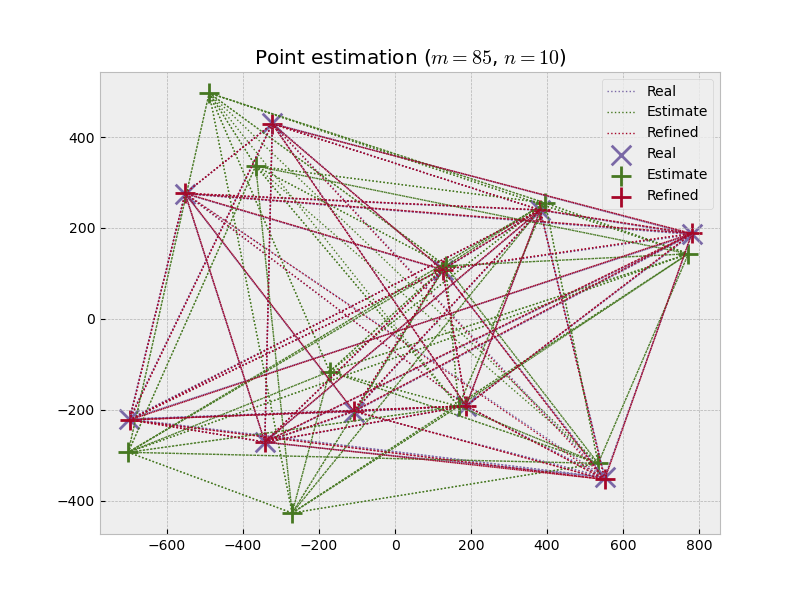
\includegraphics[width=\linewidth]{point_est_85_10.png}
    \caption{This figure shows the initial guess generated by the Riemannian elevator and the estimates after refinement, as well as the measurements between the robots.}
    \label{fig:init-ex}
\end{figure}

\subsection{Tracking}
When using the Riemannian elevator and Kruskal's method together as in algorithm~\ref{algo:estimation}, it is possible to track the robots over time. In the plots below, the tracking performance of the pipeline is displayed. 
\begin{figure}[ht]
    \centering
    \includesvg[width=\linewidth]{m90_n10_s10.svg}
    \caption{Tracking performance for $n=10$ robots with $m=90$ measurements and low noise. The real state (blue line) is followed almost perfectly. The jumps in the orientation $\theta$ is due to modulo $2\pi$ plots. }
\end{figure}
\begin{figure}
    \centering
    \includesvg[width=\linewidth]{m120_n15_s50.svg}
    \caption{Tracking performance for $n=15$ robots with $m=120$ measurements and medium noise. The real state is in blue. The positions are tracked almost perfectly, while the angle is noisy. Note that the angle plot is modulo $2\pi$.}
\end{figure}